\section{Derivação do DER e modelo relacional}
O DER representa as entidades conceituais, seus atributos identificadores, os relacionamentos e as cardinalidades. O modelo relacional deriva dessas estruturas as tabelas, chaves primárias, chaves estrangeiras e entidades associativas necessárias à implementação.

\begin{figure}[!ht]
\centering
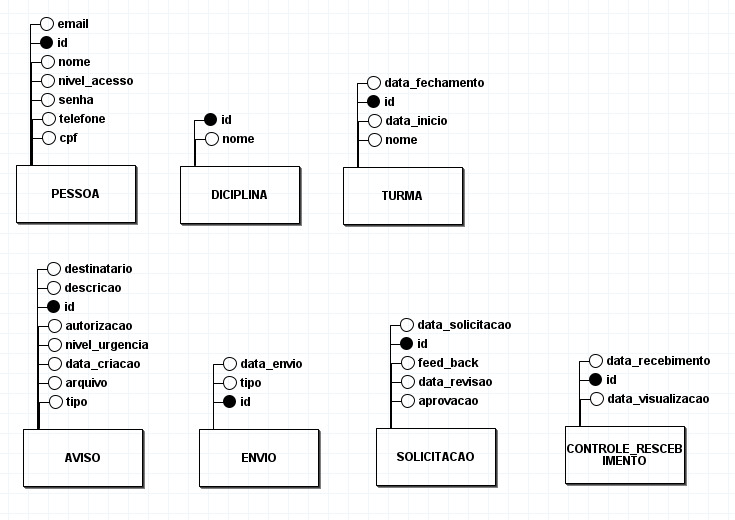
\includegraphics[width=0.95\linewidth]{../../src/uml/diagrama/der.jpeg}
\caption{DER consolidado do Sistema de Comunicação Escolar.}
\end{figure}

\begin{figure}[!ht]
\centering
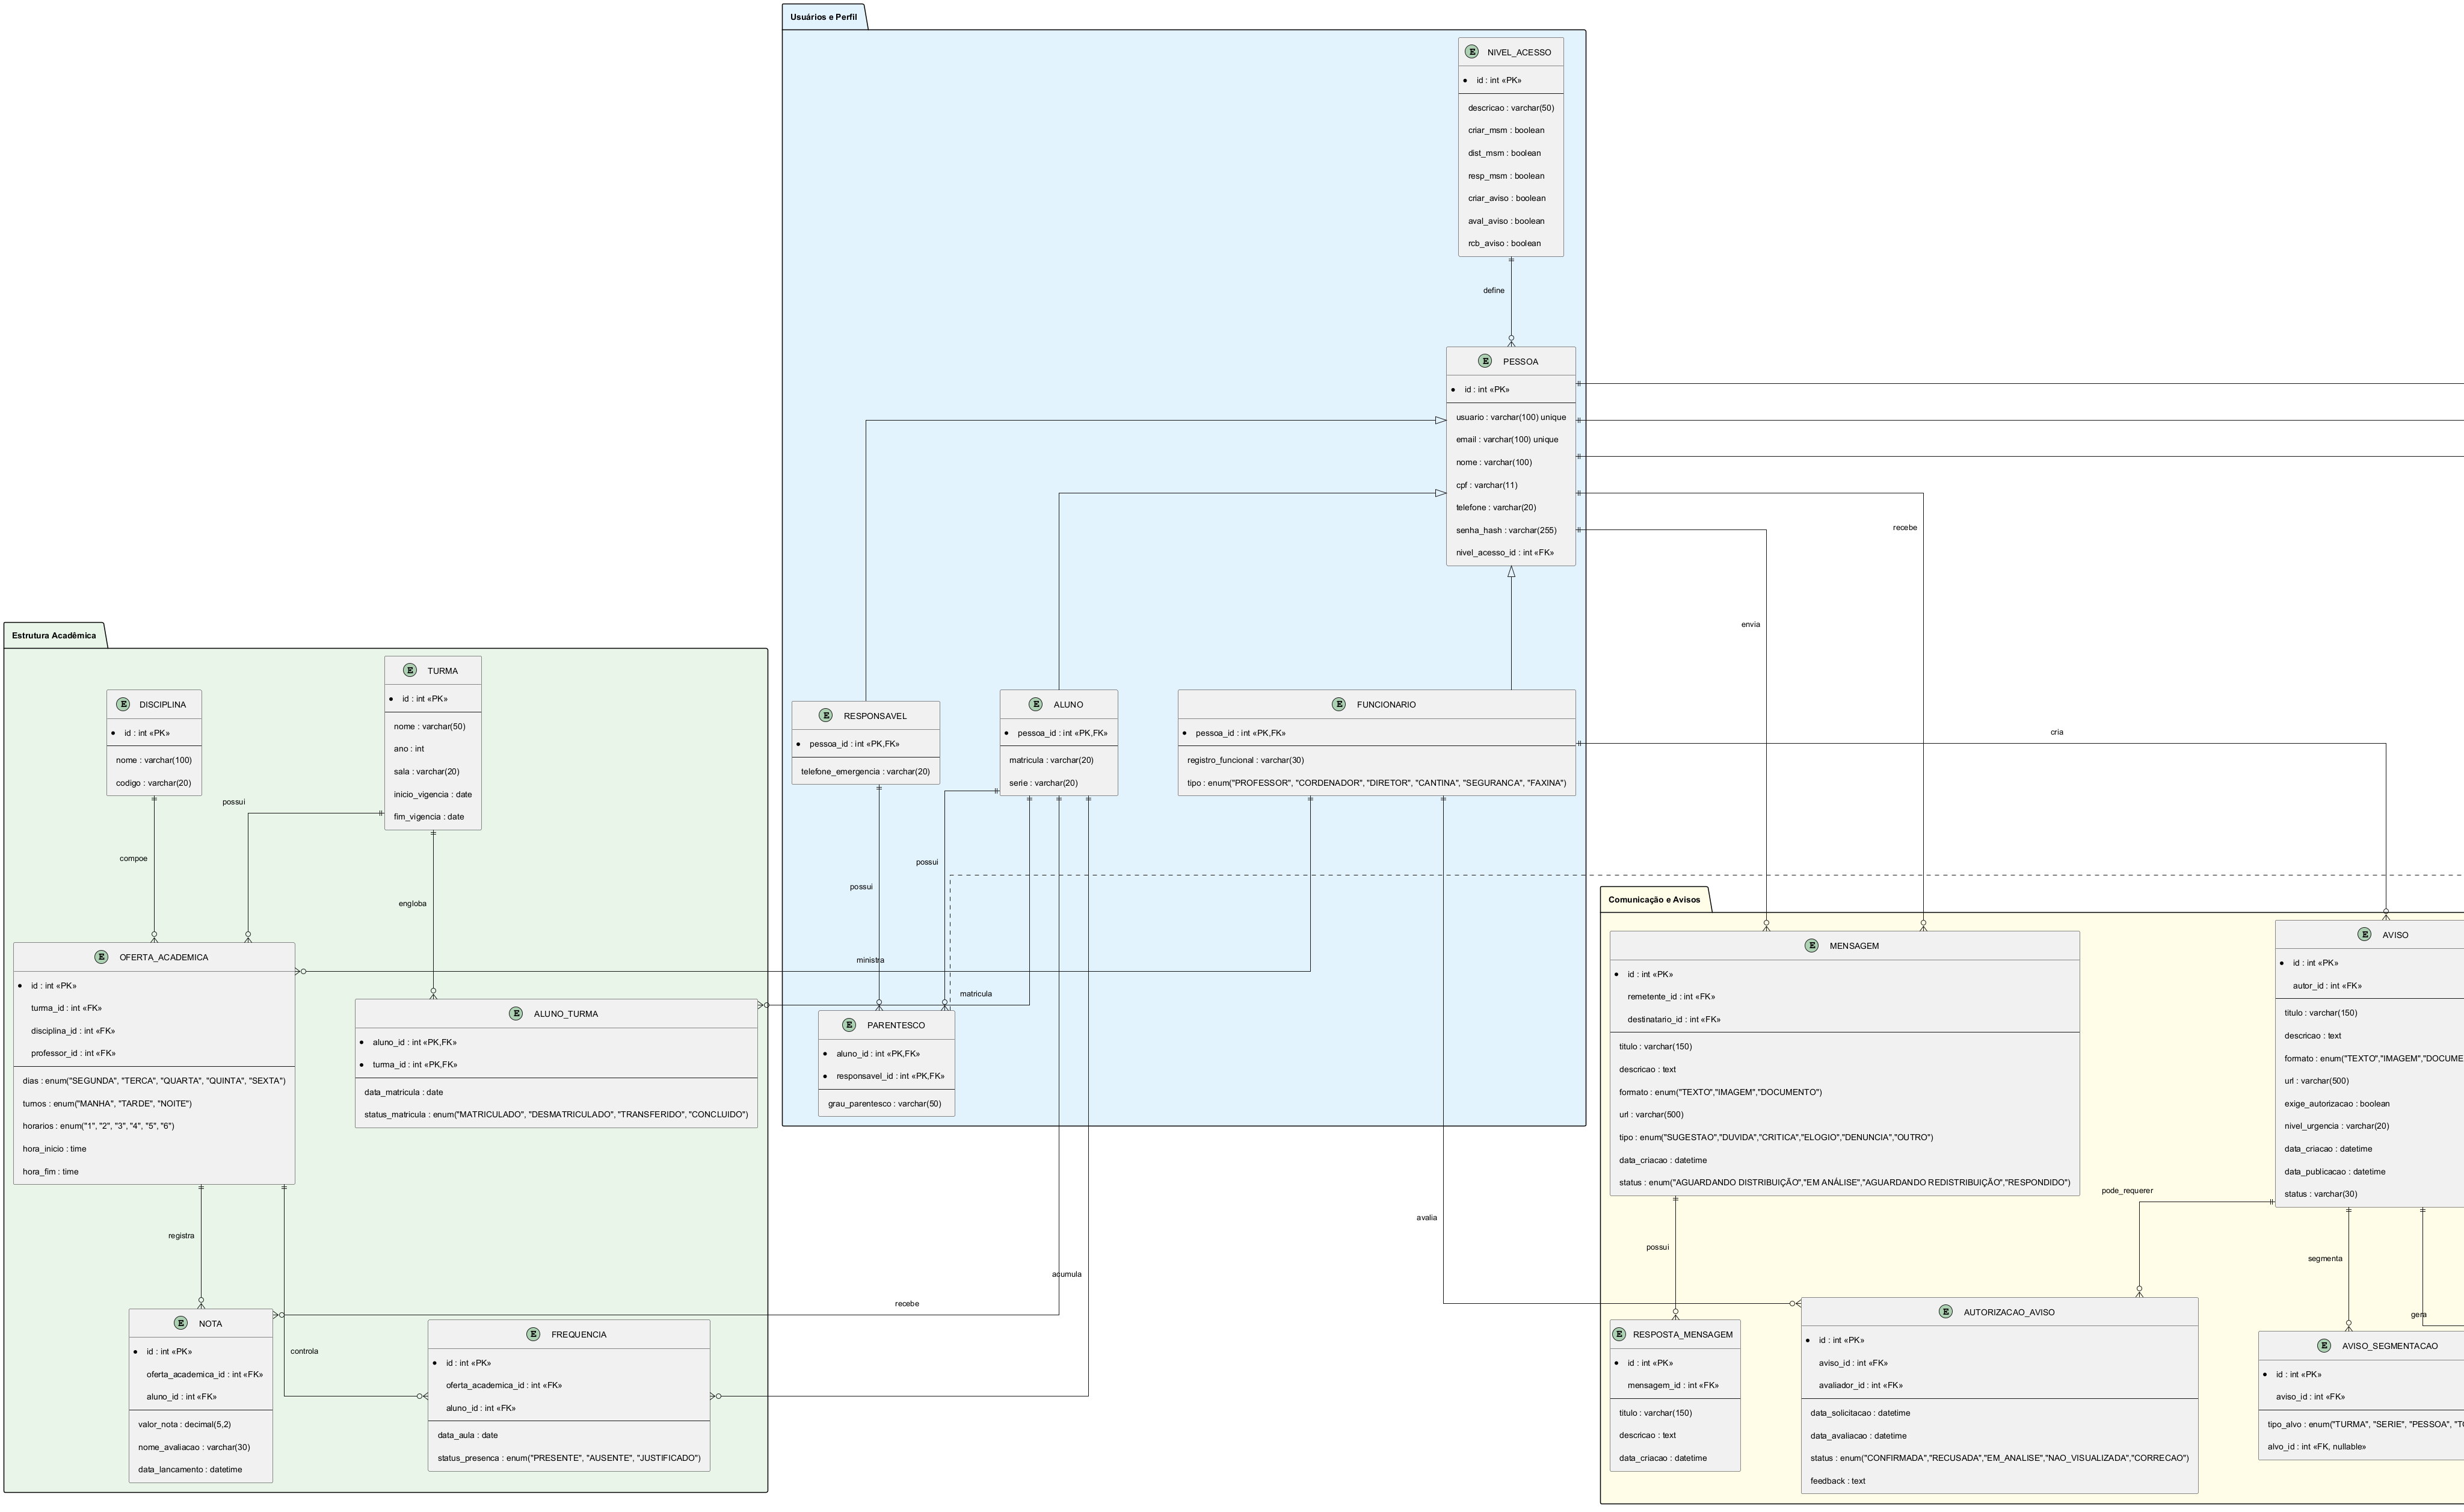
\includegraphics[width=0.95\linewidth]{../../src/uml/logico/mr.png}
\caption{Modelo Relacional do Sistema de Comunicação Escolar.}
\end{figure}
